% \documentclass[12pt]{article}
% \usepackage[utf8]{inputenc}	% Para caracteres en español
% \usepackage{amsmath,amsthm,amsfonts,amssymb,amscd}
% \usepackage{multirow,booktabs}
% \usepackage[table]{xcolor}
% \usepackage{fullpage}
% \usepackage{lastpage}
% \usepackage{enumitem}
% \usepackage{fancyhdr}
% \usepackage{mathrsfs}
% \usepackage{ textcomp }
% \usepackage{ gensymb }

% \usepackage{wrapfig}
% \usepackage{setspace}
% \usepackage{indentfirst}
% \usepackage{calc}
% \usepackage{multicol}
% \usepackage{cancel}
% \usepackage[retainorgcmds]{IEEEtrantools}
% \usepackage[margin=3cm]{geometry}
% \usepackage{amsmath}
% \usepackage{siunitx}
% \usepackage[final]{pdfpages}

% \newlength{\tabcont}
% \setlength{\parindent}{0.0in}
% \setlength{\parskip}{0.05in}
% \usepackage{empheq}
% \usepackage{framed}
% \usepackage[most]{tcolorbox}
% \usepackage{xcolor}


% \usepackage[round]{natbib}
% \bibliographystyle{plainnat}
% \colorlet{shadecolor}{orange!15}
% \parindent 0in
% \parskip 12pt
% \geometry{margin=1in, headsep=0.25in}
% \theoremstyle{definition}
% \newtheorem{defn}{Definition}
% \newtheorem{reg}{Rule}
% \newtheorem{exer}{Exercise}
% \newtheorem{note}{Note}
% \newcommand{\norm}[1]{\left\lVert#1\right\rVert}
% \doublespacing

% \newcommand{\dtoprule}{\specialrule{1pt}{0pt}{0.4pt}\specialrule{0.3pt}{0pt}{\belowrulesep}}
% \newcommand{\dbottomrule}{\specialrule{0.3pt}{0pt}{0.4pt}\specialrule{1pt}{0pt}{\belowrulesep}}
% \newcommand{\rncaps}[1]
%     {\MakeUppercase{\rncaps #1}}

\chapter{Introduction to X-ray Binary Systems and SS 433}
\section{The General Introduction and the Layout}
Understanding the physical conditions and evolution of relativistic jets from compact objects of an X-ray binary system is a challenge. SS 433 is the only source so far detected that has a pair of persistently precessing jets. Furthermore, it is the only jet source that shows spectral lines from many different elements \citep{Margon1980}. Therefore, the micro-quasar SS 433 offers an unique laboratory to probe its jet’s physical conditions. While previous radio and optical observations have given important information about the jet's motion and radiative properties, both the radio and the optical emission originates farther away than the X-ray does. Since X-ray emissions probe the most inner regions of the system (from distances \textless $4\times 10^{14}$ cm down to $\sim 10^{12}$ cm or less from the compact object \citep{Marshall2013}), they stand out to answer the fundamental questions about high energy astrophysics. What is the physical mechanism that launches the jet? How temperature and ionization state change along the jet?\par 

The project presented in this thesis is analyzing the Chandra/HETGS spectra of SS 433 getting from a 116 sec observation during August 10-14, 2018. The whole observation is split into a 20 ksec short observation 3 days before an eclipse that happened on August 10, 2018 and a 96 ksec long observation from the middle to the end of the eclipse beginning on August 13, 2018. Two phenomenological models were used to fit to the spectra from both short and long observations, which provide the redshift values and fluxes of the emission lines. A four-temperature plasma model was also fit to the data, studying the physical properties of the jet. The focus is on comparing the properties of emission lines between the short and the long observations and studying the evolution of the spectra within the long observations.





\section{X-ray binaries}
\subsection{Introduction to X-ray binaries}
An X-ray binary system consists of a compact object, which can be a black hole or a neutron star, gravitationally bounded to another star. The formation of an X-ray binary system is as follows: The more massive star in a binary will evolve more rapidly and explode as a supernova, leaving either a black hole or a neutron star. X-rays are generated in binary systems because of accretion of matter, coming from the optical companion, onto the compact objects. Therefore, the compact object is often called the accretor and the companion star is called the donor. \par 

X-ray binary systems can be divided in two different sub-classes. One of the sub-classes is the High Mass X-ray Binaries (HMXBs), where the donor is significantly more massive than the Sun. The other sub-class is the Low Mass X-ray Binaries (LMXBs) where the donor is a late - type star, with $M \leq M_\odot$. 

\subsection{Accretion Processes in X-ray Binaries}
There are two ways for the compact object to accrete material from the companion star. The first case is when either the size of the donor expands due to the nuclear fusion, or the binary separation shrinks due to the loss of angular momentum caused by gravitational radiation or magnetic braking. The Roche lobe is the region of a star within which the orbiting material is gravitationally bound to that star. The donor then fills its Roche lobe at some point and the matter flows from the donor toward the accretor through the inner Lagrangian point $L_1$ (See Figure~\ref{roche}). The inflowing material forms an accretion disc around the accretor due to the conservation of angular momentum. This process is called \textbf{Roche lobe overflow}. The second case is when the donor is a hot star contained within its Roche lobe but ejects some of its mass in the form of a stellar wind. Some of this wind is captured gravitationally by the accretor. This process is called \textbf{stellar wind accretion}.\par


The strong gravitational field of a compact object accelerates the accreting material from the donor. In the case of Roche lobe overflow, the matter that is transferred from the donor to the accretor does not land on the accretor immediately. Since the particles in the accreted material experience collisions with each other, frictional heating radiates energy away, reducing the particles' angular momentum. It allows the particle to drift inwards, driving the inward spiral. ion mechanism depends on the equipotential surfaces of inary system. The equipotential surfaces are the surfaces that share the same gravitational potential. Figure~\ref{roche} shows such surfaces for a binary system \citep{Ruffini1975}. In the figure, the two tear-drop shapes are the Roche lobes of the two stars. \par

\begin{figure}[ht]
    \centering
    
\includegraphics[width = 0.6\linewidth]{Chapters/Figures/equipotential.png}
    \caption{Roche lobes and equipotential surfaces of a binary system formed by normal star $M_1$ and a compact object $M_2$. $L_1, L_2,..., L_5$ are the Lagrange points of the system (Figure credit to Jeff Bryant)}.
    \label{roche}
\end{figure}

 
The process of the accretion onto compact objects turns out to be one of the most efficient mechanisms for converting gravitational potential energy into radiation. An order-of-magnitude calculation shows this readily. For a body of mass $M$ and radius $R_{\ast}$ the gravitational potential energy released by the accretion of a mass $m$ far away onto its surface is 
\begin{equation}
    \Delta E_{acc} = GMm/R_{\ast}
    \label{accretion}
\end{equation}

where $G$ is the gravitation constant. If the accreting body is a neutron star with radius $R_{\ast} = 20$ km, and the mass to be $M \sim M_{\odot}$, the solar mass, then the yield $\Delta E_{acc}$ is $6.63\times 10^{15}$ Joules per mass. This energy is released eventually mainly in the form of electromagnetic radiation. For comparison, consider the energy that could be released from a nuclear fusion reaction. The mass of a helium atom is about 0.8\% less than the mass of four hydrogen atoms which would combine to form a helium atom. This yields an energy of 
\begin{equation}
    \Delta E_{nuc} = 0.008 mc^2
    \label{fusion}
\end{equation}
where $c$ is the speed of light and $m$ is the mass of a helium atom. So we obtain $7.2 \times 10^{14}$ Joules per mass, which is about 10.9\% of the energy that the accretion yields. Equation~\ref{accretion} shows that the more compact of the acceting object, the greater the efficiency will be.\par

\subsection{The Components of the X-ray Binaries}
\subsubsection{The Compact Object}
Many properties such as the orbital period, magnetic field strength, and binary separation of an X-ray binary system depend on the nature of the compact object. Therefore, determining whether the compact object is a neutron star or a black is important to define those properties. A typical accreting neutron star system is an object the size of a small city (e.g. Norton) with a mass about that of the Sun but radiating in X-rays alone 10000 times the energy of the Sun. According to Equation~\ref{accretion}, the amount of accreting matter needed to produce this luminosity is about $10{^{-8}} M_{\odot}\mathrm{yr}^{-1}$. The binary nature of these systems sometimes allow us to determine the mass of the accretor by measuring the orbital velocity of the donor. The orbital velocity can be obtained by measuring Doppler shifts of the absorption lines, created by the donor.  \par

\subsubsection{The Donor}
An X-ray binary is classified as low-mass or high-mass according to the mass of the donor star. Usually, HMXBs contain a young, early-type (O, B or A), high-mass donor star which usually transfers mass by its stellar wind. LMXBs contain a late-type donor star or a white dwarf that usually undergoes Roche lobe overflow. 
%There are two non-physical approximations that give the the radius of the Roche lobe of the mass donor. They are functions of the binary mass ratio $q (=\dfrac{M_2}{M_1}) $ and separation $a$:

% \begin{

\subsubsection{The Accretion Disc}
From the previous section, we have seen that in an X-ray binary system, the accreting material usually has sufficient angular momentum to form an accretion disc. The gravitational energy gained by the gaseous matter is converted into heat, a fraction of which is converted into radiation, cooling down the accretion disc.\par 
Accretion discs in different binary systems have different properties. The discs in white dwarf binaries emit mainly in optical and ultraviolet while those in quasars and other active galactic nuclei emit radio emissions. Accretion discs that have characteristic temperatures $T\lesssim 10^6$K will radiate generally in the ultraviolet, optical and infrared \citep{King2002}. The temperatures of the inner and outer edges of an accretion disk can be determined by Keplerian orbital velocity

\begin{align}
     \dfrac{mv^2}{r} &= \dfrac{GMm}{r^2}\\
     v &= \sqrt{\dfrac{GM}{r}}
\end{align}
where $m$ is the accretion mass, $M$ is the mass of the accretor, $r$ is the distance from the accretion mass to the accretor,
and the equipartition theorem
\begin{equation}
    \dfrac{1}{2}mv^2 \sim \dfrac{3}{2}kT
\end{equation}
where $k$ is the Boltzmann constant.
For an X-ray binary system, the inner edge of the the accretion disk is could have a radius $R_{\mathrm{in}} \sim 10$ km and a temperature $T_{\mathrm{in}} \sim 10^7$ K. The outer edge of the disk could have $R_{\mathrm{in}} \sim 10^6 $ km and $T_{\mathrm{in}} \sim 10^3$ K \citep{King2002}. 
Figure~\ref{bhbinary} shows sketch of 16 Milky Way black hole binaries with companion stars and the accretion disks drawn to scale.\par


\begin{figure}[ht]
    \centering
    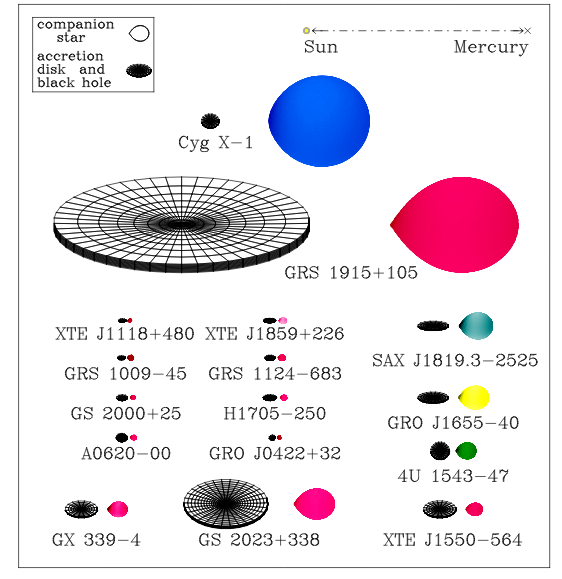
\includegraphics[width = 0.7\textwidth]{Chapters/Figures/BH_binaries.png}
    \caption{Scale drawings of 16 black hole binaries in the Milky Way (Figure by Jerome Arthur Orosz). The Sun–Mercury distance (0.4 AU) is shown at the top. The color of the companion star approximately indicates its surface temperature.}
    \label{bhbinary}
\end{figure}

\subsection{Maximum Luminosity during accretion: The Eddington Limit}

If the star has luminosity $L$ and radius $R$, the radiation pressure acting on an electron on the star's surface is
\begin{equation}
    -\dfrac{\sigma_T F}{c} = \dfrac{\sigma_T L}{4\pi R^2c},
\end{equation}
where $F$ is the incident radiation from the star and $\sigma_T$ is the Thomson cross section:
\begin{equation}
    \sigma_T = \dfrac{8\pi}{3}(\dfrac{e^2}{m_e c^2})^2 = 6.65 \times 10^{-25} \mathrm{cm^2}
\end{equation}
The maximum luminosity during a spherical accretion is attained when the inward gravitational force on a hydrogen atom balances out the outward pressure of radiation
\begin{equation}
    \dfrac{\sigma_T L_{\mathrm{edd}}}{4\pi R^2c} = \dfrac{GMm_p}{R^2}
\end{equation}
where $G$ is the gravitational constant, $c$ is the speed of light, $M$ is the mass of the gravitating body, $m_p$ and $M_{\odot}$ are the mass of the proton and the mass of the Sun. The luminosity at this point is called \textbf{Eddington luminosity},  also referred to as the Eddington limit 
\begin{equation}
    L_{Edd} = \dfrac{4\pi GMm_pc}{\sigma_0} = 1.26\times 10^{38} (\mathrm{M/M_{\odot}) erg/s} = 1.26\times 10^{31} (\mathrm{M/M_{\odot}) Joules/s}
    \label{eddington}
\end{equation}
Accretion discs are not spherical and often have additional stresses, related to turbulence, viscosity, shear and magnetic fields \citep{Pringle1981, Balbus1998}. Those additional stresses can counteract the radiation pressure along with gravity. Therefore, accretion discs may be somewhat brighter than the Eddington limit and radiate at super-Eddington luminosity. \par

\subsection{Jets}
Astronomical jets are collimated outflows moving at relativistic speed. The first jet discovered was of M87 in optical photographs from Lick Observatory by Heber Curtis in 1918. Figure~\ref{m87} shows later optical, radio, and X-ray images of M87 taken by the Hubble Space Telescope (HST), the Large Array radio telescope (VLA) and the Chandra telescope. The irregular, knotty structure in X-ray image of the jet is similar to that detected by radio telescopes and the Hubble Space Telescope. At the very left of the images we see the bright galactic nucleus harboring a supermassive black hole.\par 

\begin{figure}[ht]
    \centering
    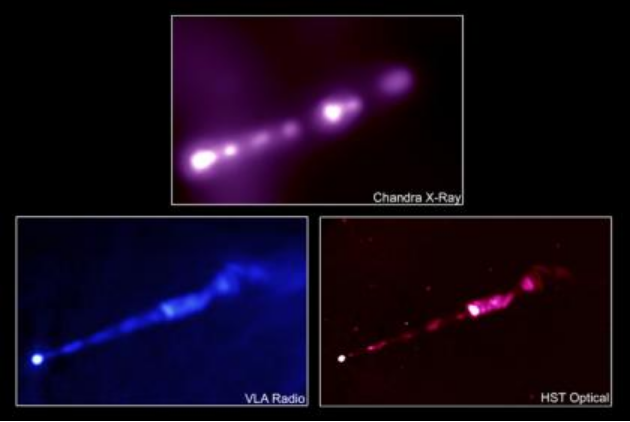
\includegraphics[width = 0.7\textwidth]{Chapters/Figures/M87jet.png}
    \caption{M87 jets observed by telescopes at X-ray, radio, and optical wavelengths. Top: X-ray image using Chandra telescope (NASA/CXC/MIT/H.Marshall et al.). Bottom left: Radio map take by the VLA (F. Zhou, F.Owen (NRAO), J.Biretta (STScI)). Bottom right: Optical image taken by HST (NASA/STScI/UMBC/E.Perlman et al.).  }
    \label{m87}
\end{figure}

Jets may consist of particles (mostly likely electrons and/or protons) moving at speeds close to the speed of the light (relativistic speed). The details of the formation of the powerful jets are still unclear. Jets can have significant impact on the surrounding matter. The jet that emanates from one galaxy can interact with the companion galaxy. This interaction may cause or inhibit the star formation.\par 

Inside the jet where the temperature is high, the collisions between atoms excite electrons into higher energy levels. When the electron decay back to its ground state in a very short of time (typically $10^{-8}$ s), it releases energy in the form of photon of a characteristic wavelength. This causes the bright emission lines in the spectrum. While it takes only $\sim 10^4$ K to completely ionize hydrogen, it is hard to completely ionize heavy elements such as iron and magnesium because they have many electrons. Thus only at very high temperature regions, such as the parts of the jet that are closest to the accretor of an X-ray binary system, would those heavy atoms be ionized to a higher degree. Magnetic field in the accretor causes those free high-speed electrons spirals around magnetic field lines of force, creating the radio, optical and X-ray knots \citep{Miller_2002}. Then electrons start to emit radiation as they accelerate in the magnetic field, which is called the \textbf{synchrotron radiation}. Another process that produces photons in the jets is  \textbf{Bremsstrahlung radiation}, which is radiation produced by a charged particle, undergoing acceleration. Bremsstrahlung radiation forms the continuum X-ray spectrum.



\section{Introduction to SS 433}

SS 433 is the first discovered microquasar. It is a smaller version of quasar that is composed of a compact object with a mass several times that of our sun and a companion star. SS stands for the initials of two astronomers, C.B. Stephenoson and N. Sanduleak, who compiled a list of emission-line objects \citep{Stephenoson1977}. SS 433 is the 433rd entry in that list. SS 433 is near the center of a supernova remnant called W50, a large nebula elongated in east-west direction. Figure~\ref{w50} shows W50, which has the shape similar to a conch. Due to the radio impact of W50, the coordinate of SS 433 was mistakenly identified several times. The realization that the radio, optical, and X-ray emissions are actually from the same object, SS 433, was reached by \cite{Clark1978}.\par

\begin{figure}[ht]
    \centering
    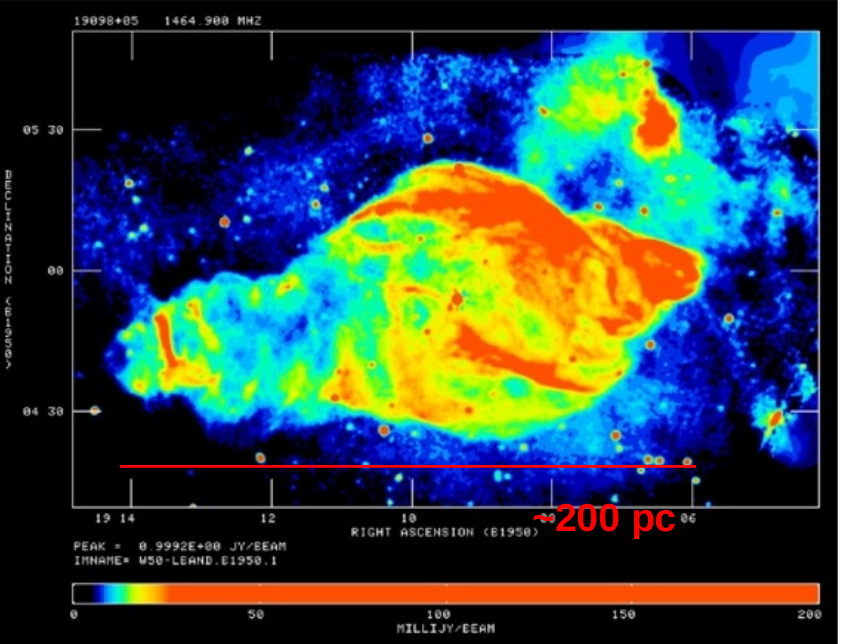
\includegraphics[width = .8\linewidth]{Chapters/Figures/w50.png}
    \caption{A radio map produced by VLA showing SS 433 as radio star surrounded by the shell of the W50 nebula. The big red dot near the center indicates SS 433 \citep{Dubner1998}.}
    \label{w50}
\end{figure}


\subsection{The moving lines}
SS 433 is one of the many emission-line objects showing very strong H$\alpha$ (the 3 to 2 transition in hydrogen) and neutral helium (He I) emission lines in the optical spectrum. Other than these emission lines, the spectrum of SS 433 contains many bright emission features at unfamiliar wavelengths. However, there are two other emissions for each rest line at abnormal wavelengths moving from one night to the next. The velocity of the changing motion is astonishing comparing to other binary systems. This caused the attention of Bruce Margon and his colleagues \citep{Margon1979}. They found that many other emission lines also have moving components. Each line's sets of components move in the same pattern (Figure~\ref{dopplershift}). It shows the smooth periodic motion of the pair of lines in opposite directions.

\begin{figure}[ht]
    \centering
    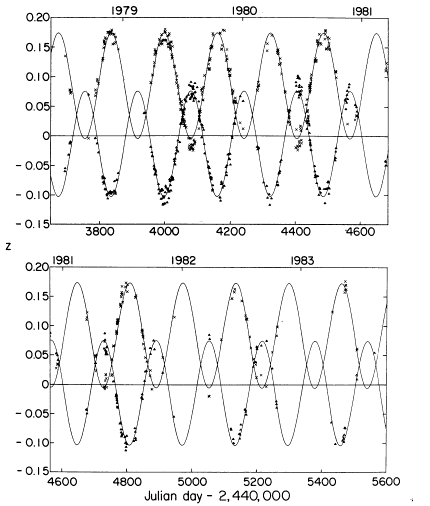
\includegraphics[scale = 0.6]{Chapters/Figures/dopplershift.png}
    \caption{Doppler shifts of SS 433 on 450 nights in the period 1978-1983. The period is the 164 days, showing the stability of the periodic motion of the jets. \citep{Margon1984}.}
    
    % The solid curve is a least-squares best fit to the kinematic model. The free parameters and their associated 1$\sigma$ uncertainties for this fit are $v/c = 0.2601\pm$0.0014, $\theta=19.80\degree \pm 0.18\degree$, $i = 78.82\degree \pm0.11\degree$, $P_p = 162.532 \pm 0.062$ days.
    \label{dopplershift}
\end{figure}

There were two conjectures associated with this motion of the lines if we assumed that it is due to the orbiting motion of two bodies. Firstly, the amplitude of the movement is enormous, which indicates a maximum velocity of about 50,000 km s$^{-1}$ in the redshifted and a minimum velocity of 30,000 km s$^{-1}$ in the blueshifted feature \citep{Margon1984}. From Kepler's law, in order to have such large velocity, the orbiting object in the binary needs to have a mass of about a billion times of the Sun. It is quite impossible that human did not detect such massive object in the galaxy \citep{seward_charles_2010}.\par 

Secondly, the average velocity of the motion is about 12000 km s$^{-1}$. Assuming a cosmological origin for this velocity (and using Hubble's constant which is $\sim$ 70 km/s/Mpc), SS 433 would be extremely far away from us (definitely extragalactic). However, the stationary emission lines are at a much lower velocity, which suggests that it is located within our galaxy \citep{seward_charles_2010}. 

\subsection{Relativistic jets}
The solution to solve the mystry of the `moving lines' is the \textit{kinematic model}
developed independently by \cite{Fabian1979} and \cite{Milgrom1979}. Abell and Margon fitted this model to the optical characteristics of SS 433 \citep{Margon1979}. The solid lines in Figure~\ref{dopplershift} is a least-squares best fit to the kinematic model. This model consists of a pair of jets of gas travelling in opposite directions at a relativistic speed of 0.26$c$ \citep{Margon1979}. Figure~\ref{geomtry_ss433} shows the geometry of the SS 433 system. Two jets precess about a common axis with the 164-day period. Therefore, the pair of jets vary their orientation respect to us from time to time, causing the observed Doppler velocity modulation. There are times when both jets are travelling perpendicular to our line of sight and then the moving lines appear to cross over in the spectrum (Figure~\ref{dopplershift}).\par 


\begin{figure}[ht]
    \centering
    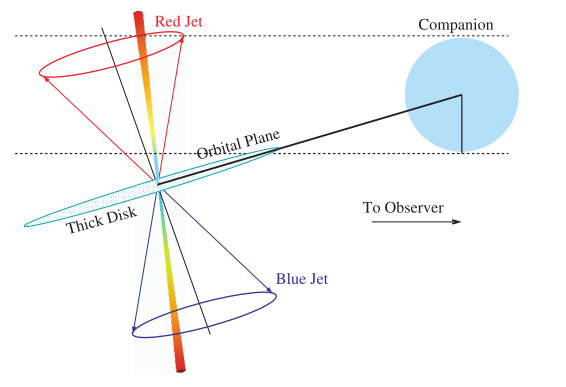
\includegraphics[width = 0.7\linewidth]{Chapters/Figures/geometry_ss433.png}
    \caption{Schematic geometry of the `kinematic model' of SS 433. This shows a pair of jets moving in opposite directions. The opening angle of the jet $\theta=19.80\degree \pm 0.18\degree$. The angle between the jet axis and the line of sight is $i = 78.82\degree \pm0.11\degree$. The period of the jet precession is $P_p = 162.532 \pm 0.062$ days \citep{Margon1984}. Figure from \citep{Lopez2006}.}
    \label{geomtry_ss433}
\end{figure}

At the times when both lines are crossing, the value of the redshift is not zero. It is due to the fact of special relativity. Imagine a object is travelling at an angle $\theta$ to our line of sight with velocity $v$. The component of this velocity toward us is $v\mathrm{cos}\theta$. According to the classical Doppler shift, when $v$ is small, any radiation emitted with a wavelength $\lambda_0$ will be observed by us at a wavelength $\lambda$ where
\begin{equation}
    \lambda = \lambda_0\left(1+\dfrac{v\mathrm{cos}\theta}{c}\right).
    \label{nonrelativistic_doppler}
\end{equation}
We notice that when $\theta = 90$, $\lambda = \lambda_0$, which means that when the object is moving perpendicular to us, there will be no Doppler effect. The observed wavelength shift (redshift) value is defined by 
\begin{equation}
    z = \dfrac{\lambda - \lambda_0}{\lambda_0} = \dfrac{v\mathrm{cos}\theta}{c}
\end{equation}
But when $v$ is very large, in the sense of a large fraction of the speed of light $c$, the effect of special relativity needs to be considered. The observed wavelength now becomes
\begin{equation}
    \lambda = \lambda_0 \dfrac{1 + \dfrac{v\mathrm{cos\theta}}{c}}{\left(1 - \dfrac{v^2}{c^2}\right)^{1/2}}
    \label{relativistic_doppler}
\end{equation}
Notice that Eq(\ref{relativistic_doppler}) reduces to Eq(\ref{nonrelativistic_doppler}) when $v \ll c$. \par 

This is called the \textbf{relativistic Doppler shift}. The principle is that if two clocks are synchronized and one is moving in a spacecraft relative to the other on the Earth at a large speed, the observer on the earth will observe the clock on the spacecraft slower compared to one on the Earth. This is called the \textbf{time dilation}, which is independent of the direction in which the spacecraft is travelling. The clock will appear to run slow no matter whether the spacecraft is travelling toward, away from you or perpendicular to the line of sight. For a spectral line, it is similar to an atomic clock in the sense that it appears to run ``slow'' when it moves at relativistic speed. This dilation applies to the duration between two successive light wave crests emitted by the source. Therefore, the observed wavelength is always greater than the emitted one. The factor by which it does run slow is the $\left(1 - \dfrac{v^2}{c^2}\right)^{1/2}$ shown in Equation ~\ref{relativistic_doppler}, which is called the \textit{Lorentz gamma factor}. According to Equation~\ref{relativistic_doppler} and Figure~\ref{dopplershift} which shows $z(\theta = 90\degree) = 0.035$, the velocity of the jet is 0.26$c$.\par
As seen from the earth the jet that is more Eastern oriented approaches us most of the time, we called it the blue jet. Similarly, we call the other jet, which is more Western oriented and receding from us most of the time, the red jet. 


\subsection{SS 433 as an X-ray binary} 
Combining the angular periodicity of the corkscrew structure projected on the plane of the sky produced by the precession of the jet axis, and the jet velocity of 0.26c, the distance to SS 433 is determined to be 5.5 kpc \citep{Blundell2004}. 
From the spectrum of SS 433, in addition to the fast moving emission lines from the jet, there are also slowly moving features from the donor star that have a period of 13.1 days \citep{Crampton1980}, which is the period of the this binary system. Tentative detections of donor's spectrum have been made \citep{Hillwig2004} showing that the mass donor is probably an early-typed A supergiant star (A3-7 I) with a temperature between 7,500 to 10,000 K. Over an estimate of forty years, the range of the mass of the compact object have spanned from 1 to 30 solar masses \citep{Bowler2018}, from neutron star to massive stellar black hole. It is still unclear which is correct although recent studies \cite{Lopez2006} and \cite{Bowler2018} point to a black hole of mass of $15 \pm 2 M_{\odot}$. The dilemma of determining the mass ratio could be resolved if the spectrum of the companion could be identified and its orbital velocity curve measured. In \cite{Bowler2018}, the ratio of the mass of compact object to the mass of the companion star is calculated to be about 0.7 based on the shape of the He I stationary lines. \par

The absolute magnitude of SS 433 is $-6^m.28 < M_V < -5^m.4$ \citep{Goranskij2011}, the interstellar extinction $A_v$ in the direction of SS 433 is $7^m.3 - 8^m.3$ \citep{Cherepashchuk1982} and distance of the system $d$ is 5.5 kpc. We can then predict the apparent V-band magnitude $m_V$ of the donor according to the distance modulus formula
\begin{equation}
    m_V = M_V - 5 + 5\mathrm{log}_{10}(d) + A_V.
\end{equation}
The predicted apparent V-band magnitude is calculated to be about $15^m.9$. However, the observed apparent V-band magnitude is $13^m$ \citep{Cherepashchuk1982}. This discrepancy suggests that SS 433 exceeds the Eddington luminosity.\par


\subsection{The Uniqueness of SS 433}
Many more microquasars have been discovered since the discovery of SS 433. Most of them are black hole X-ray transients, whose intensities vary a lot during a short amount of time. However, SS 433 is the only source that has a pair of persistently precessing jets. Furthermore, it is the only jet source that shows spectral lines from many different elements \citep{Margon1980}. Thus, we know that SS 433's jet is made of baryonic matter, i.e. heavy particles, such as protons and neutrons \citep{seward_charles_2010}. The moving lines produced by those elements indicate the precise velocity (0.26$c$) of the jet, and line diagnostics give the temperature and density.\par 

The observed super-Eddington luminosity is quite likely the result of much higher mass transfer rate in SS 433 ($10^{-4} M_{\odot} \mathrm{yr}^{-1}$) than other known HMXBs \citep{Van_den_heuvel1981}. This may imply that SS 433 is a short-lived binary system, with a lifetime of a few tens of thousands of years only \citep{seward_charles_2010}. That may be a reason why microquasar like SS 433 is so rare in the universe.




\subsection{X-ray Observations of SS 433}
The early X-ray observations (e.g. using EXOSAT/GSPC, ASCA) showed that the strongest X-ray emission line was caused by highly ionized iron which lost all but one of its electrons (Fe {\sc xxvi}) \citep{Watson1986}. This indicates that the X-ray emission must originate in inner region of the system, which has a high temperature of $50-100 \times 10^6$ K \citep{fabrika2004}. The total luminosity of the X-ray emission is $L_x$ is from $3 \times 10^{28} - 10^{29} \mathrm{J/s}$ \citep{fabrika2004}. X-ray emission is strongly variable. It depends on the orientation of the accretion disk and jets (precessional phase) and the effects of eclipses of the optical star (orbital phase). The detected X-ray iron lines in those observations are from the Eastern (approaching) jet but lines are absent from the Western (receding) jet \citep{fabrika2004}. The reason could be the receding jet is eclipsed by the accretion disk (indicated in Figure~\ref{geomtry_ss433}).\par

Previous studies on the X-ray observation of SS 433 have been published by \cite{Marshall2002}, \cite{Lopez2006}, and \cite{Marshall2013}, focusing on studying SS 433 with Chandra High Energy Transmission Grating Spectrometer (discussed in Chapter 2). \cite{Marshall2002} resolved the X-ray lines, detected fainter lines than previously observed. \cite{Lopez2006} utilized an eclipse to determine the radius of the companion star, which is $1.08 \times 10^{12} $ or $15.50 R_{\odot}$. \cite{Marshall2013} observation used an eclipse to conclude that the X-ray spectra were remarkably consistent before and after the eclipse and eclipsed emission is hard. It also suggests that the directions of the Eastern and Western jets are independently determined or affected by the environment. Figure~\ref{HETG2002} shows Chandra's high spectral resolution, which allows studying the X-ray emission lines of SS 433 in more details than was possible earlier. In most of the Chandra HETG observations, there are many lines from the approaching jet and a few lines from the receding jet. The strongest line was a helium-like line of iron Fe \rncaps{25} \citep{Marshall2002, Marshall2013}.


\begin{figure}[h!]
    \centering
    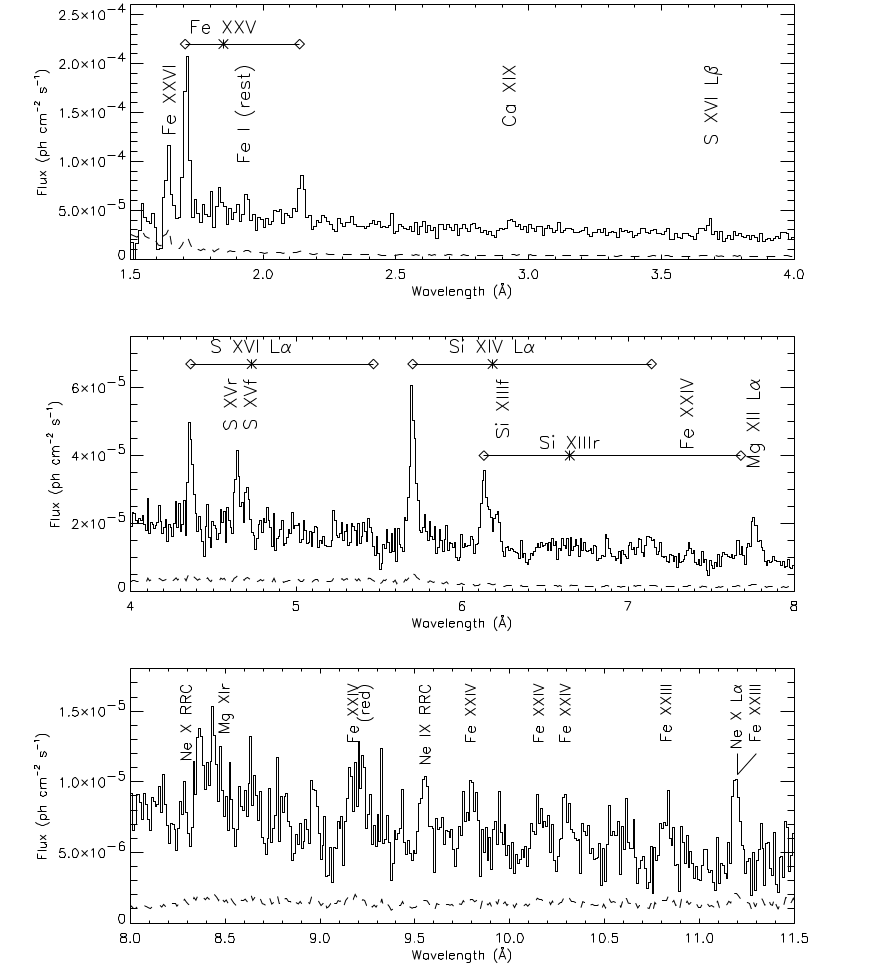
\includegraphics[width = \linewidth]{Chapters/Figures/HETG2002.png}
    \caption{Chandra HETGS spectrum of SS 433 obtained at precession phase 0.51 and orbital phase 0.67. Most of the lines are from the blue jet. The strongest lines are marked with horizontal bar indicating the positions of the red-shifted, blue-shifted (diamonds) and rest wavelengths (asterisks) (original diagram by \citep{Marshall2002}.}
    \label{HETG2002}
\end{figure}

Three Si {\sc xiii} lines (Si {\sc xiii} triplets) whose rest wavelengths at 6.2 \AA\ region are used to determine the electron density. These three lines are called  Si {\sc xiii}r,  Si {\sc xiii}i, and  Si {\sc xiii}f. Letter r, i, and f indicate ``resonance'', ``intercombination'', and ``forbidden'' respectively \citep{porquet2010}. Figure~\ref{HETG2002} shows lines from Si\rncaps{13}f and Si\rncaps{13}r. They are the most intense lines of helium-like ions (``triplet''). They correspond to transitions between n= 2 shell and n= 1 ground-state shell \citep{porquet2010}. In Figure~\ref{rif}, resonance is shown as $w$, which is an electric dipole transition, intercombination as $x + y$, which is a magnetic quadrupole transition and forbidden as $z$ transition, which is a relativistic magnetic dipole transition \citep{porquet2010}.



\begin{figure}[h!]
    \centering
    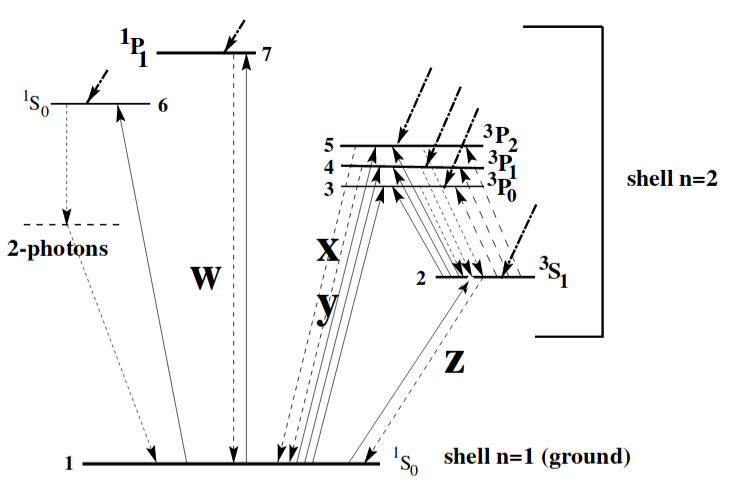
\includegraphics[width = 0.7\linewidth]{Chapters/Figures/rifgraph.png}
    \caption{Simplified level scheme for helium-like ions w (or resonance) x; y (or intercombination), and z(or forbidden): resonance, intercombination, and forbidden lines, respectively \citep{porquet2010}.}
    \label{rif}
\end{figure}







\section{Some unanswered questions about the jets of SS 433}
Previous detailed spectral modeling shows that there is a broad range of temperatures in the outflow, with different ionization states sampling different regions of the jets. Although previous observations provided valuable insights about the jets, none of these observations were designed to follow the source while it was coming out of an eclipse. Therefore, using an eclipse of the compact object by the donor, our 96 ksec long observation tracking the accretor coming out of the eclipse can map out the spatial variations of the physical properties of SS 433’s X-ray jet. Splitting the spectrum from the long observation into 5 parts and analyzing them enable us to see how the flux of the emission lines, redshifts of the jets, and other physical properties of the jets change over the long observation. These information will give us insights about which regions of the jets produce certain kind of elements. What is more, the 20 ksec short observation taken before an eclipse enables us to check that the changes in line properties during the main observation were indeed due to the eclipse and not due to any significant changes in the intrinsic accretion in/outflows. Previous observations were all taken when the Western jet (which points away from us most of the time) was receding from us, which causes the Western jet being too faint to analyze. Our observation, instead, were designed to take during the epochs when the Western jet was closest to our line-of-sight and hence easiest to observe due to Doppler beaming. \cite{Marshall2013} observation suggests that the Doppler shifts change by $\gtrsim 3000 km \mathrm{s^{-1}}$ during the day. This suggests that the two jets might be moving independent to each other. Therefore, we would also like to check whether there was another abnormal change of the redshift during our observation. \par 




% Knowing more about which lines are occulted by the eclipse will help us understand better about the geometry of the system, which is helpful to estimate the size of the companion star. Those information would further benefits to estimate the masses of both the accretor and the donor. 




 













% \subsection{The Radio jets and W50}
% SS 433 is a very bright radio star, whose central radio source radiates at a level of about 1 Jy (a non-SI unit non-SI unit of spectral flux density, equivalent to about $10^-26$ watts per square meter per Hz) at centimeter wavelengths. The maximum of the radio emission occurs at a distance of $\sim 10^15$ cm from the source \citep{Hjellming1981}, the same place where the strongest optical jet line emission originates. The brightness of the radio jet decreases to a distance of $\sim 10^17$ cm away from the source and became invisible beyond this distance until a distance of $\sim 10^{20}$ cm. At this place, the jets are decelerated and the large-scale X-ray jets are observed together with an increased intensity of the radio emission \citep{}.








%\subsection{The disc and Precession Mechanism}

%-----------------------------------

%----------------------------









